%   =============================
%		Change document settings here 
%   =============================

% TITLEPAGE SETTINGS
% ------------------
\newcommand{\docAutor}				{various}								% name of the author of the book
\newcommand{\docTitel}				{Algorithms I}			% title of the lecture/book
\newcommand{\docUntertitel}			{Lecture Notes of Spring 2013}		% subtitle
\newcommand{\docDozent}				{tbd}			% name of the professor
\newcommand{\docJahr}				{2013}			% publishing year
\newcommand{\docUniversitaet}	{University of Mannheim}	% name of university
\newcommand{\docTitelZitat}		{}
\newcommand{\docTitelZitatName}	{}				% titlepage quote author

% GENERAL SETTINGS
% ----------------
\newcommand{\useIndex}					{0} 											% set '1' if you want to include an index
\newcommand{\useThumbs}					{0}												% set '1' if you want to use chapter thumbs on the page side
\newcommand{\useRoman}					{0}												% set '1' if you want to have chapter numbering with roman numbers

\newcommand{\usrBCOR}					{0cm}    										% set binding correction offset here (space lost on the inner borders due to binding)
\newcommand{\usrmatter}					{0}												% set '1' to start numbering at actual content beginning
\newcommand{\usroptsqrt}				{1}												% set '1' to use alternate form for roots with a small closing line
\newcommand{\usrnscmd}[1]				{\textbf{#1}}							% set e.g. '\textbf', '\mathbb' or '\mathds' for namespace macros
				% document specific settings

\documentclass[a4paper, 						% paper size
							 12pt, 								% font size
							 BCOR = \usrBCOR,			% binding correction
							 DIV=15, 							% used for typearea calculation
							 headsepline,					% add head line to border calculation
							 twoside, 						% two-sided document
							 footnotes = multiple,% visually separate two consecutive footnotes
							 toc = index,					% add index to table of contents
							 numbers = auto,			% automatic placing of end dot in numbering
							 pagesize							% used for flexibility
							]{scrbook}						% KOMA book class
							
% PREAMBLE
% =========
					
\usepackage[english]{babel}
\usepackage[latin1]{inputenc}					% input encoding
\usepackage[T1]{fontenc}							% use T1 fonts for font encoding
\usepackage{amsfonts}									% math font
\usepackage{newcent}									% use New Century Schoolbook
\usepackage{fouriernc}								% math font for newcent
\usepackage{dsfont}										% math font for number spaces etc.
\usepackage{helvet}										% sans serif font
\usepackage{inconsolata}							% font for typewriter style

% general
\usepackage{makeidx}
\makeindex

\usepackage{ifthen}
\usepackage{letltxmacro}							% better support for redefining macros with optional arguments
\usepackage{booktabs}									% nicer tables
\usepackage{wrapfig}									% text around figures
\usepackage{parskip}									% vertical space instead of indentation
\usepackage{microtype}								% improved justification
\usepackage{needspace}								% reserve space
\usepackage{framed}										% shaded environments
\setlength{\FrameSep}{0pt}						% correct colorbox width (package: framed)

\usepackage{xcolor}
\usepackage{graphicx}
\usepackage{tikz}
\usetikzlibrary{positioning}
\usetikzlibrary{arrows}

\usepackage{enumitem}
\setenumerate[1]{label=\roman*)}			% roman numbered lists
\setitemize			{leftmargin=*}
\setenumerate		{leftmargin=*}


\usepackage{chapterthumb}							% use chapter thumbs
\setkomafont{chapterthumb}						% use small font for chapter thumbs
	{\normalfont\sffamily}
\renewcommand{\chapterthumbheight}		% make chapter thumbs thinner
	{1em}
	
\setkomafont{chapterentry}						% no sans-serif but bold chapter entries in toc
	{\normalfont\bfseries}
\setkomafont{chapterentrypagenumber}	% no bold chapter page entry numbers in toc
	{\normalfont}
	
\renewcommand{\footnoterule}{					% increase spacing below footnote line
	\noindent\rule{0.4\textwidth}{.4pt}
	\vspace{0.6em}}
\deffootnote{1em}{1em}								% footnote in normal textsize
	{\thefootnotemark\hspace{0.5em}}
	
\usepackage{scrpage2}
\setkomafont{pageheadfoot}
	{\normalfont\itshape}
\pagestyle{scrheadings}								% switch to modified style

\renewcommand{\chaptermark}[1]
	{\markboth{\thechapter~#1~}{}}
\renewcommand{\sectionmark}[1]
	{\markright{\thesection\autodot~#1}}
					
\usepackage{titlesec}									% design chapter headings
\titleformat{\chapter}[display]
	{\normalfont\sffamily\Huge\bfseries\flushright\fontsize{70}{0}\selectfont}
	{\thechapter}
	{-0pt}{\Huge}
\setkomafont{section}{\normalfont\Large\bfseries}
\setkomafont{subsection}{\normalfont\large\bfseries}
\titlespacing*{\chapter}{0pt}{0pt}{50pt}

\ifthenelse{\equal{\useRoman}{1}}									% roman chapter numbering
	{\renewcommand{\thechapter}{\Roman{chapter}}}{}
					
\clubpenalty 					= 10000					%
\widowpenalty 				= 10000					% avoid widow and club lines
\displaywidowpenalty 	= 10000					%

\makeatletter
\@beginparpenalty			=	10000					% avoid page breaks before lists
\makeatother

\definecolor{linkblue}{rgb}{0.0, 0.0, 0.3}
\definecolor{citeblue}{rgb}{0.0, 0.0, 0.5}
\usepackage[pdfstartpage				= 1,							% default opening start page 
						pdfstartview				= FitB, 					% default opening zoom
						pdftitle						= {\docTitel},		% document title
						pdfauthor						= {\docAutor}, 		% document author
						colorlinks					= true, 					% print links colored
						bookmarks						= true, 					% use bookmarks
						bookmarksopen				= true,						% open bookmarks by default
						bookmarksnumbered		= true, 					% number bookmarks
						linkcolor						= linkblue,					% color for links
						citecolor						= citeblue,				% color for cite links
						pdfdisplaydoctitle	= true						% display document title instead of file name
					 ]{hyperref}

% mathematical
\usepackage{amssymb}
\usepackage{amsmath}
\usepackage{amsthm}
\usepackage{latexsym}
\usepackage{stmaryrd}
\usepackage{esint}										% provides \ointclockwise etc.
\usepackage{mathtools}								% provides \xRightarrow[]{}, \mathclap, \shortintertext and \bigtimes

\makeatletter																			% alternate closed root symbol
\ifthenelse{\equal{\usroptsqrt}{1}}{%
\let\oldr@@t\r@@t
\def\r@@t#1#2{%
\setbox0=\hbox{$\oldr@@t#1{#2\,}$}\dimen0=\ht0
\advance\dimen0-0.2\ht0
\setbox2=\hbox{\vrule height\ht0 depth -\dimen0}%
{\box0\lower0.65pt\box2}}
\LetLtxMacro{\oldsqrt}{\sqrt}
\renewcommand*{\sqrt}[2][\ ]{\oldsqrt[#1]{#2}}}{}
\makeatother				% general settings and packages
\newcommand{\A}{\usrnscmd A}
\newcommand{\B}{\usrnscmd B}
\newcommand{\C}{\usrnscmd C}
\newcommand{\D}{\usrnscmd D}
\newcommand{\E}{\usrnscmd E}
\newcommand{\F}{\usrnscmd F}
\newcommand{\G}{\usrnscmd G}
%\renewcommand{\H}{\usrnscmd H}						% only activate if needed
\newcommand{\I}{\usrnscmd I}
\newcommand{\J}{\usrnscmd J}
\newcommand{\K}{\usrnscmd K}
%\renewcommand{\L}{\usrnscmd L}						% only activate if needed
\newcommand{\M}{\usrnscmd M}
\newcommand{\N}{\usrnscmd N}
%\renewcommand{\O}{\usrnscmd O}						% only activate if needed
%\renewcommand{\P}{\usrnscmd P}						% only activate if needed
\newcommand{\Q}{\usrnscmd Q}
\newcommand{\R}{\usrnscmd R}
\renewcommand{\S}{\usrnscmd S}
\newcommand{\T}{\usrnscmd T}
\newcommand{\U}{\usrnscmd U}
\newcommand{\V}{\usrnscmd V}
\newcommand{\W}{\usrnscmd W}
\newcommand{\X}{\usrnscmd X}
\newcommand{\Y}{\usrnscmd Y}
\newcommand{\Z}{\usrnscmd Z}

\newcommand{\sA}{\mathcal A}
\newcommand{\sB}{\mathcal B}
\newcommand{\sC}{\mathcal C}
\newcommand{\sD}{\mathcal D}
\newcommand{\sE}{\mathcal E}
\newcommand{\sF}{\mathcal F}
\newcommand{\sG}{\mathcal G}
\newcommand{\sH}{\mathcal H}
\newcommand{\sI}{\mathcal I}
\newcommand{\sJ}{\mathcal J}
\newcommand{\sK}{\mathcal K}
\newcommand{\sL}{\mathcal L}
\newcommand{\sM}{\mathcal M}
\newcommand{\sN}{\mathcal N}
\newcommand{\sO}{\mathcal O}
\newcommand{\sP}{\mathcal P}
\newcommand{\sQ}{\mathcal Q}
\newcommand{\sR}{\mathcal R}
\newcommand{\sS}{\mathcal S}
\newcommand{\sT}{\mathcal T}
\newcommand{\sU}{\mathcal U}
\newcommand{\sV}{\mathcal V}
\newcommand{\sW}{\mathcal W}
\newcommand{\sX}{\mathcal X}
\newcommand{\sY}{\mathcal Y}
\newcommand{\sZ}{\mathcal Z}

\newcommand{\deftxt}[1]											% emphasize newly defined terms
	{\textcolor{def_color}{#1}}

\renewcommand{\I}{\mathrm i}								% imaginary unit
\newcommand{\dd}{\mathrm d}									% differential
\newcommand{\e}{\varepsilon}								% nicer epsilon
\newcommand{\id}{\operatorname{id}}					% identity operator
\newcommand{\ind}{\textbf{1}}								% indicator function
\newcommand{\norm}[1]{\left\|#1\right\|}		% norm
\renewcommand{\Re}{\operatorname{Re}}				% real part
\renewcommand{\Im}{\operatorname{Im}}				% imaginary part

% statistic-related
\newcommand{\Pois}{\operatorname{Pois}}			% Poisson distribution
\newcommand{\Var}{\operatorname{Var}} 			% variance
\newcommand{\Cov}{\operatorname{Cov}}				% covariance
\newcommand{\Binom}{\operatorname{B}}				% binomial distribution
\newcommand{\Bias}{\operatorname{Bias}}	% predefined macros
\definecolor{def_color}					{HTML}{194D6C}
\definecolor{def_shade_color}		{HTML}{DFE9EF}
\definecolor{thm_color}					{HTML}{2F2512}
\definecolor{thm_shade_color}		{HTML}{FFF7D4}	

\newlength{\internalindent}
\setlength{\internalindent}		% defines how much text and lists are intended
	{.5cm}
	
\newtheoremstyle{thmstyle}
	{\internalindent}
	{\internalindent}{
		\addtolength{\leftskip}	{\internalindent}					 
		\addtolength{\rightskip}{\internalindent}
	}
	{0pt}{}{}
	{\newline}
	{\textcolor{thm_color}{\textbf{#1} #2} \quad  \textbf{#3}}
	
\newtheoremstyle{defstyle}
	{\internalindent}
	{\internalindent}{
		\addtolength{\leftskip}	{\internalindent}					 
		\addtolength{\rightskip}{\internalindent}
	}
	{0pt}{}{}
	{\newline}
	{\textcolor{def_color}{\textbf{#1} #2} \quad  \textbf{#3}}
	
\newtheoremstyle{bspstyle}
	{\internalindent}
	{\internalindent}{
		\addtolength{\leftskip}	{0pt}					 
		\addtolength{\rightskip}{0pt}
	}
	{0pt}{}{}
	{\newline}
	{\textbf{#1} #2 \quad  \textit{#3}}
	
\theoremstyle{thmstyle}
\newtheorem{tmp_satz}{Theorem}[chapter]
\newtheorem{tmp_kor}{Korollar}[chapter]
\newtheorem{tmp_lemma}{Lemma}[chapter]
\newtheorem{tmp_prop}{Proposition}[chapter]

\theoremstyle{defstyle}
\newtheorem{tmp_def}{Definition}[chapter]

\theoremstyle{bspstyle}
\newtheorem{tmp_bsp}{Example}[chapter]
\newtheorem*{tmp_bsp*}{Example}

\newenvironment{theorem}[1][]{
	\setlist			{rightmargin=\internalindent}
	\setitemize		{leftmargin=\leftmargin}
	\setenumerate	{leftmargin=\leftmargin+\internalindent}
	\definecolor{shadecolor}{named}{thm_shade_color}
	\needspace{4\baselineskip}
	\begin{shaded}\begin{tmp_satz}[#1]
}{
	\end{tmp_satz}
	\end{shaded}
	\noindent\ignorespacesafterend
}
	
\newenvironment{korollar}[1][]{
	\setlist			{rightmargin=\internalindent}
	\setitemize		{leftmargin=\leftmargin}
	\setenumerate	{leftmargin=\leftmargin+\internalindent}
	\definecolor{shadecolor}{named}{thm_shade_color}
	\needspace{4\baselineskip}
	\begin{shaded}\begin{tmp_kor}[#1]
}{
	\end{tmp_kor}
	\end{shaded}
	\noindent\ignorespacesafterend
}

\newenvironment{lemma}[1][]{
	\setlist			{rightmargin=\internalindent}
	\setitemize		{leftmargin=\leftmargin}
	\setenumerate	{leftmargin=\leftmargin+\internalindent}
	\definecolor{shadecolor}{named}{thm_shade_color}	
	\needspace{4\baselineskip}
	\begin{shaded}\begin{tmp_lemma}[#1]
}{
	\end{tmp_lemma}
	\end{shaded}
	\noindent\ignorespacesafterend
}
	
\newenvironment{proposition}[1][]{
	\setlist			{rightmargin=\internalindent}
	\setitemize		{leftmargin=\leftmargin}
	\setenumerate	{leftmargin=\leftmargin+\internalindent}
	\definecolor{shadecolor}{named}{thm_shade_color}
	\needspace{4\baselineskip}
	\begin{shaded}\begin{tmp_prop}[#1]
}{
	\end{tmp_prop}
	\end{shaded}
	\noindent\ignorespacesafterend
}
	
\newenvironment{definition}[1][]{	
	\setlist			{rightmargin=\internalindent}
	\setitemize		{leftmargin=\leftmargin}
	\setenumerate	{leftmargin=\leftmargin+\internalindent}
	\definecolor{shadecolor}{named}{def_shade_color}
	\needspace{4\baselineskip}
	\begin{shaded}\begin{tmp_def}[#1]
}{
	\end{tmp_def}
	\end{shaded}
	\noindent\ignorespacesafterend
}

\DeclareRobustCommand{\bspendmark}{% defines end mark for examples
	\ifmmode \quad\sslash
	\else	\hbox{$\sslash$}
	\fi
}

\newenvironment{example}[1][]{	
	\pushQED{\bspendmark}
	\needspace{4\baselineskip}
	\begin{tmp_bsp}[#1]
}{
	\end{tmp_bsp}
	\noindent\ignorespacesafterend
}

\newenvironment{example*}[1][]{	
	\pushQED{\bspendmark}
	\needspace{4\baselineskip}
	\begin{tmp_bsp*}[#1]
}{
	\end{tmp_bsp*}
	\noindent\ignorespacesafterend
}
	
\renewcommand*\proofname{Proof}
\makeatletter
\newenvironment{prooof}[1][\proofname]{
	\par
	\normalfont \topsep6\p@\@plus6\p@\relax
	\trivlist
	\item[\hskip\labelsep
		\bfseries #1\@addpunct{:}]~%\newline\ignorespaces
}{
	\endtrivlist\@endpefalse
	\noindent\ignorespacesafterend
}
\makeatother

\newsavebox{\informationbox}
\newenvironment{information}
{\begin{center}\begin{lrbox}{\informationbox}\begin{minipage}{0.7\textwidth}\small}
{\end{minipage}\end{lrbox}
\begin{tikzpicture}

\draw[fill] (-0.5*\wd\informationbox - 1cm, 0.1cm) circle (0.3cm);
\draw[color=white] (-0.5*\wd\informationbox - 1cm, 0.1cm) node {\large\bfseries i};

\draw (0,0) node {\usebox{\informationbox}};
\end{tikzpicture}\end{center}
}

\newcommand{\boffset}{7pt}			% space the frame surrounds the text
\newcommand{\bthickness}{1pt}
\newcommand{\blength}{4*\bthickness}
\newsavebox{\chapdescbox}
\newenvironment{descr}
{\begin{center}\begin{lrbox}{\chapdescbox}\begin{minipage}{0.9\textwidth}}
{\end{minipage}\end{lrbox}
\begin{tikzpicture}
	\draw[fill] (-0.5*\wd\chapdescbox - \boffset - \bthickness, \ht\chapdescbox + \boffset + \bthickness) 	rectangle
							(-0.5*\wd\chapdescbox - \boffset							, \ht\chapdescbox + \boffset - \blength);
	\draw[fill]	(-0.5*\wd\chapdescbox - \boffset - \bthickness, \ht\chapdescbox + \boffset + \bthickness) 	rectangle
							(-0.5*\wd\chapdescbox - \boffset + \blength		, \ht\chapdescbox + \boffset);
							
	\draw[fill]	(0.5*\wd\chapdescbox + \boffset								, -\dp\chapdescbox - \boffset - \bthickness) 	rectangle
							(0.5*\wd\chapdescbox + \boffset + \bthickness	, -\dp\chapdescbox - \boffset + \blength);
	\draw[fill]	(0.5*\wd\chapdescbox + \boffset + \bthickness	, -\dp\chapdescbox - \boffset) 								rectangle
							(0.5*\wd\chapdescbox + \boffset - \blength		, -\dp\chapdescbox - \boffset - \bthickness);
	
	\draw (0,0) node {\usebox{\chapdescbox}};
\end{tikzpicture}\end{center}
}
		% predefined environments
%
% define how to hyphenate certain words in case you're experiencing problems with them
% use the following command pattern:
% \hyphenation{hy-phe-na-te}
%
		% custom hyphenation rules

%\includeonly{}											% while writing your book, compile only what you need

\begin{document}
\raggedbottom
\ifthenelse{\equal{\usrmatter}{1}}
	{\frontmatter}{}
\begin{titlepage}
\raggedleft
{\large \docAutor\\[1in]}
{\large \docUntertitel\\[.2in]}
{\fontsize{35}{0}\selectfont\bfseries\docTitel\\[.2in]}
\ifthenelse{\equal{\docTitelZitat}{}}{}
{{\footnotesize{\itshape \docTitelZitat}\\\docTitelZitatName\\}}
\vfill
{\large \docUniversitaet\\\docJahr}
\end{titlepage}

\newpage
\thispagestyle{empty}

\markboth{Legal Notes}{Legal Notes}

\noindent This script originates from the course "`\docTitel"' at the University of Mannheim as lecture notes.

The accuracy of its content is not guaranteed and the author(s) do not assume responsibilitty for possible damages of any kind.
This lecture notes are not an official document released by employees of the University of Mannheim, hence those do not assume responsibility, as well.

Many thanks to Ingo B�rk, who initially published the underlying LaTeX template \href{http://www.matheboard.de/thread.php?threadid=498961}{here}.
This work is licensed under a \href{http://creativecommons.org/licenses/by-nc-sa/3.0/de/deed.en_US}{Creative Commons Attribution-NonCommercial-ShareAlike 3.0 Germany License}.
\newpage
\tableofcontents
\ifthenelse{\equal{\usrmatter}{1}}
	{\mainmatter}{}
\ifthenelse{\equal{\useThumbs}{1}}
	{\ihead[\putchapterthumb]{\putchapterthumb}}{}
	
% ================================
% include your document parts here
% only use section-wise documents since include inserts new pages!
\chapter{TODO: 1st lecture missing}

\begin{descr}
    TODO
\end{descr}

\section{TODO}\index{TODO}
\begin{definition}
    TODO
\end{definition}
\begin{definition}
    TODO
\end{definition}
\begin{definition}
    TODO
\end{definition}
\begin{lemma}
    TODO
\end{lemma}

\begin{definition}
    Let $G = (V,E)$ be a graph without loops. If there exists $V_{1}, V_{2} \leq V$ and $V_{1} \cup V_{2} = V$
    such that $V_{1} \cap V_{2} = \emptyset$ and every edge $e$ has one endpoint in $V{_1}$ and the other in $V_{2}$,
    then we call $G$ a \deftxt{bipartite}.
\end{definition}

\begin{example*}
    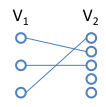
\includegraphics{diagrams/def14_example1.png}
\end{example*}

\begin{definition}
    A directed graph is a pair $G = (V,E)$ where $V$ is a set of nodes (vertices) and $E$ is a set of edges together 
    with a function $i: E -> V x V$. If $i(e) = (v_{1},v_{2})$ then $v_{1}$ is called start point, $v_{2}$ is called end point.
\end{definition}
Graphically: \\[3mm]
If $i(e) = (v_{1},v_{2})$ we draw 1. \\
If $i(e') = (v_{1},v_{2})$ then this indices a second edge (2.). \\
If $i(e_{1}) = i(e_{2})$ we call $e_{1},e_{2}$ parallel. \\
If $i(e) = (v,v)$ then $e$ is called a directed loop. \\
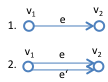
\includegraphics{diagrams/def15_directd_graph.png} \\
$g_{out}(v)$ is the number of edges that have starting point $v$. \\
$g_{in}(v)$ is the number of edges with endpoint $v$.

\begin{lemma}
    $\displaystyle\sum\limits_{v \in V} g_{in}(v) = \displaystyle\sum\limits_{v \in V} g_{out}(v)$
\end{lemma}

\begin{prooof}
    We start with a graph without edges. Then we insert one after the other edges in $E$. 
    Each edge contributes 1 to both sides of the equation.
\end{prooof}

\begin{definition}
    A directed path is a sequence of edges $e_{1},e_{2}...$ such that the end point of $e_{i}$ is the start point of
    $e_{1} +1, i > 1$([NW] +1 seems strange to me, correct?). \\[3mm]

    A directed path $e_{1}...e_{k}$ is called a (directed) \underline{cycle}, if the start point of $e_{1}$ and
    the end point of $e_{k}$ coincide. \\
    A simple (directed) path is a path where every node occurs at most once. \\
    A directed cycle is called simple if every node except for the start and end node occurs at most once.
\end{definition}

\begin{definition}
    A graph directed or undirected is called \underline{simple}, if it does not contain parallel edges.
\end{definition}

\begin{definition}
        A directed graph is called \underline{strongly connected} if for any pair of nodes $(u,v)$ 
        there is a directd path from $u$ to $v$.
\end{definition}

Let $G$ be a directed graph $G = (V,E)$. $x,y \in V x~y$ ([NW] does ~ mean are "connected"?)
if there is a directed path from x to y and vice versa. \\

The equivalence classes of this relation $~c VxV$ are called strongly connected components.
(Analogously: Define connected components for undirected graphs)

\begin{information}
    We should know how the following terms are defined: reflexivity, symetry, transitivity.
\end{information}



	\section{Einstellungen zu Rechtshinweisen, Vorwort und Titelseite}

Die Dateien des sogenannten \verb|frontmatter|-Bereiches\footnote{Falls dieser �ber den \texttt{\textbackslash usrmatter}-Schalter (siehe \ref{sec:einstellungen}, \ref{var:usrmatter}) �berhaupt verwendet wird. Andernfalls existiert er zwar dennoch, erh�lt aber keine separate Nummerierung.} im Ordner \verb|inc/| sollten an die eigenen Anspr�che angepasst werden. Dies umfasst die folgenden Dateien:
\begin{enumerate}
	\item \verb|copyright.tex| -- f�r die Lizenzbestimmungen. Als Standard ist eine "`Creative Commons"'-Lizenz eingestellt.
	\item \verb|preface.tex| -- f�r das Vorwort des Buches. Hier kann der Inhalt des Buches zusammengefasst, auf das Thema hingeleitet oder das Thema motiviert werden. Das Vorwort sollte keinesfalls aus mehreren Unterkapiteln bestehen oder andersweitig Merkmale aufweisen, die den Charakter des Inhaltes besitzen.
	\item \verb|titlepage.tex| -- f�r die Titelseite. In der Regel sollte diese Datei nicht ver�ndert werden, es sei denn, es ist explizit ein anderes Titelseitenlayout erw�nscht.
\end{enumerate}


	\section{Einstellungen}\index{Einstellungen}\label{sec:einstellungen}

In der Datei \verb|inc/settings/settings.tex| finden sich alle wichtigen Einstellungen, die von dieser Vorlage angeboten werden, um das Layout oder Verhalten zu bestimmen. Unge�bten \LaTeX-Anwendern wird empfohlen, nur diese Einstellungen zu variieren und f�r �nderungen innerhalb der Vorlage Hilfe zu konsultieren, um unerw�nschte Effekte zu vermeiden. Manche Schalter nehmen lediglich die Werte \verb|0| und \verb|1| an\footnote{Tats�chlich kann man ihnen beliebige Werte zuweisen, lediglich der Wert \texttt{1} aktiviert den Schalter jedoch.}. Der Wert \verb|1| aktiviert, der Wert \verb|0| deaktiviert den entsprechenden Schalter.

An dieser Stelle wollen wir im Detail auf die einzelnen Schalter und Optionen in der eben erw�hnten Datei eingehen:
\begin{enumerate}
	\item \verb|\docAutor|, \verb|\docTitel|, \verb|\docUntertitel|, \verb|\docDozent|, \verb|\docJahr|, \verb|\docUniversitaet| -- mit diesen Befehlen wird die Ausgabe auf der Titelseite\footnote{In der Standarddatei f�r die Rechtshinweise werden diese Befehle ebenfalls verwendet.} gesteuert und automatisch angepasst.
	\item \verb|\docTitelZitat|, \verb|\docTitelZitatName| -- diese beiden Befehle betreffen ebenfalls die Titelseite. Es kann ein Zitat angegeben werden, das standardm��ig unter dem Titel erscheint. Aufgrund der unterschiedlichen Formatierung wird der Name der zitierten Person getrennt gespeichert. Der Befehl darf jedoch auf keinen Fall gel�scht werden, sondern muss einfach mit einem leeren Inhalt definiert werden.
	\item \verb|\useIndex| -- mit diesem Schalter kann festgelegt werden, ob ein Stichwortverzeichnis ausgegeben werden soll.
	\item\label{var:usethumbs} \verb|\useThumbs| -- dieser Schalter aktiviert kleine K�stchen am rechten Seitenrand, die bei gedruckter Form helfen, bequem das richtige Kapitel aufzuschlagen. Es gilt jedoch zu beachten, dass nur wenige Drucker den Rand wirklich bedrucken k�nnen.
	\item \verb|\useRoman| -- Mit dieser Einstellung werden Kapitel, die mit \verb|\chapter| er�ffnet werden, mit r�mischen statt arabischen Ziffern nummeriert.
	\item \verb|\usrBCOR| -- da beim Binden eines Buches Teile des inneren Randes augenscheinlich verschwinden wird die Bindekorrektur (BCOR, engl. \emph{binding correction}) eingef�hrt.
	\item\label{var:usrmatter} \verb|\usrmatter| -- ist diese Option aktiviert, so werden die Seiten vor dem eigentlichen Inhalt des Buches separat nummeriert und in r�mischen Zahlen ausgegeben. Die Nummerierung beginnt ab dem eigentlichen Inhalt dann neu.
	\item \verb|\usroptsqrt| -- mit diesem standardm��ig aktiviertem Schalter wird die Form des Wurzelsymbols angepasst, so dass ein schlie�ender Strich eingef�gt wird: $\sqrt{x}$ versus $\oldsqrt{x}$ % Anmerkung: Der Befehl \oldsqrt wird hier nur zur Demonstrationszwecken verwendet; von einer Anwendung im Dokument ist dringend abzuraten!
	\item\label{var:usrnscmd} \verb|\usrnscmd| -- hier wird der Befehl eingestellt, der f�r die Zahlenraum-Makros \verb|\A|, \ldots, \verb|\Z| verwendet wird (siehe \ref{sec:makros}). Eine g�ngige Alternative ist \verb|\mathbb|, sch�ner w�re jedoch \verb|\mathds|. Als Standard wird eine simple Fettschrift gesetzt, da dies auch der traditionellen Form entspricht.
\end{enumerate}

	\section{Verf�gbare Makros}\index{Makros}\label{sec:makros}

Diese Vorlage bietet standardm��ig bereits viele vordefinierte Makros und Umgebungen. Die Definitionen der Makros werden in der Datei \verb|inc/settings/abbreviations.tex| verwaltet. Je nach pers�nlichen Pr�ferenzen und der Notwendigkeit kann diese vordefinierte Liste ver�ndert oder erweitert werden.
\begin{information}
Makros sind ein wichtiges Werkzeug, um einen konsistenten Stil zu gew�hrleisten. Sie erleichtern zudem die Arbeit, da etwaige �nderungen nur einmalig und nicht m�hsam im gesamten Dokument durchgef�hrt werden m�ssen.
\end{information}

An dieser Stelle wollen wir alle verf�gbaren Makros kennenlernen:
\begin{enumerate}
	\item Die Befehle \verb|\A|, \ldots, \verb|\Z| liefern Buchstaben f�r Zahlenr�ume, lediglich \verb|\H|, \verb|\L|, \verb|\O| und \verb|\P| stehen nicht standardm��ig zur Verf�gung. Der Befehl \verb|\I| ist ebenfalls andersweitig belegt (siehe \ref{makro:im}). Es existieren nur Gro�buchstaben mit diesen Befehlen. Die Makros verwenden intern den Befehl \verb|\usrnscmd|\footnote{Siehe \ref{sec:einstellungen}, \ref{var:usrnscmd}.}, der standardm��ig auf \verb|\textbf| eingestellt ist.
	\begin{align*}
	\A, \B, \C, \D, \E, \F, \G, \J, \K, \M, \N, \Q, \R, \S, \T, \U, \V, \W, \X, \Y, \Z.
	\end{align*}
	Weit verbreitet sind auch die Befehle \verb|\mathbb| und \verb|\mathds| f�r doppelgestrichene Buchstaben. Historisch gesehen wurden diese aber nur eingef�hrt, da Fettschrift an der Tafel schwer umzusetzen war, weswegen diese Varianten eigentlich nicht verwendet werden sollten. Da sie dennoch sehr verbreitet sind werden sie unterst�tzt. Es wird empfohlen, in diesem Fall \verb|\mathds| zu verwenden, da die Doppelstriche an der korrekten Position sind und die Schriftzeichen die richtige Gr��e haben.
	\item Analog liefert \verb|\sA|, \ldots, \verb|\sZ| kalligrafisch geschwungene Buchstaben. Auch hier gibt es nur Gro�buchstaben, es existieren hierbei aber sogar alle Buchstaben. Intern verwendet wird der Befehl \verb|\mathcal|.
	\begin{align*}
	\sA, \sB, \sC, \sD, \sE, \sF, \sG, \sH, \sI, \sJ, \sK, \sL, \sM, \sN, \sO, \sP, \sQ, \sR, \sS, \sT, \sU, \sV, \sW, \sX, \sY, \sZ.
	\end{align*}
	\item Mit dem Befehl \verb|\deftxt{\ldots}| k�nnen definierte Begriffe hervorgehoben werden.\\
	\verb|Wir nennen dies einen \deftxt{Begriff}| liefert:
	\begin{align*}
	\text{Wir nennen dies einen \deftxt{Begriff}}
	\end{align*}
	\item\label{makro:im} F�r die imagin�re Einheit $\I$ existiert das Makro \verb|\I|.
	\item F�r das Differential $\dd$ in Integralen steht das Makro \verb|\dd| zur Verf�gung.
	\item F�r das h�ufig verwendete $\e$ gibt es den Befehl \verb|\e|.
	\item Mit \verb|\id| erh�lt man den Identit�tsoperator $\id$.
	\item F�r die Indikatorfunktion kann \verb|\ind_A(x)| verwendet werden und liefert dann $\ind_A(x)$.
	\item Eine Norm kann mit \verb|\norm{x}| geschrieben werden und liefert $\norm{x}$. Die Normstriche passen sich in der Gr��e automatisch an.
	\item Der Realteil $\Re z$ und der Imagin�rteil $\Im z$ komplexer Zahlen lassen sich mit \verb|\Re z| und \verb|\Im z| notieren, verhalten sich also genauso wie die g�ngigen Operatoren wie z. B. \verb|\sin x| f�r $\sin x$.
	\item F�r Notationen der Stochastik existieren \verb|\Var| f�r die Varianz $\Var$, \verb|\Cov| f�r die Kovarianz $\Cov$ und \verb|\Pois| f�r die Poisson-Verteilung $\Pois$.
\end{enumerate}
	\section{Verf�gbare Umgebungen}\index{Umgebungen}

Nachdem wir nun die Makros kennen, die von der Vorlage bereitgestellt werden, kommen wir zu den verf�gbaren Umgebungen. Ihre konsequente Verwendung wird f�r einen typographisch guten Stil dringend empfohlen:
\begin{enumerate}
	\item Definitionen k�nnen mit der \verb|definition|-Umgebung erstellt werden.\\
	\verb|\begin{definition} \ldots \end{definition}| liefert:
	\begin{definition}
	\ldots
	\end{definition}
	Die Nummerierung erfolgt automatisch entsprechend des aktuellen Kapitels. Alle Umgebungen teilen sich einen "`Z�hler"', so dass jede Nummer einzigartig ist.
	\item F�r S�tze, Korollare, Lemmata und Propositionen gibt es entsprechende Umgebungen verm�ge \verb|satz|, \verb|korollar|, \verb|lemma| und \verb|proposition|. Analog zu der \verb|definition|-Umgebung liefert dies beispielsweise:
	\begin{satz}[Satz von \ldots]
	\ldots
	\end{satz}
	\item F�r Beispiele stehen die Umgebung \verb|beispiel| bzw. \verb|beispiel*| f�r unnummerierte Beispiele zur Verf�gung:
	\begin{beispiel}
	\ldots
	\end{beispiel}
	Endet ein Beispiel beispielsweise in einer Liste oder in einer abgesetzten Gleichung, so kann mit \verb|\qedhere| der Endmarker manuell an die entsprechende Stelle gesetzt werden.
\end{enumerate}
All diese Umgebungen erlauben zudem einen optionalen Parameter in eckigen Klammern -- also z. B. \verb|\begin{satz}[Bezeichnung]| --, welcher f�r den Titel der Umgebung gew�hlt wird. Je nach Umgebung kann dies eine Bezeichnung des Theorems oder der zu definierende Begriff sein. Ein Beispiel hierf�r wurde eben schon gezeigt.

\begin{information}
Die Umgebungen sichern sich mit Hilfe des \verb|needspace|-Pakets bereits Platz, dennoch kann es unter Umst�nden zu leichten Darstellungsfehlern kommen, bei denen oben oder unten der Leerraum zum farbigen Hintergrund fehlt. Dieser Fehler l�sst sich bisher leider nur durch redaktionelle Eingriffe im Einzelfall beheben.
\end{information}

\begin{enumerate}[resume]
	\item F�r Beweise steht die \verb|beweis|-Umgebung zur Verf�gung. Ihr Aussehen ist schlicht gehalten. Das \verb|\qed|-Symbol wird automatisch eingef�gt; sollte der Beweis jedoch mit einer abgesetzten Gleichung enden, so sollte der Befehl \verb|\qedhere| innerhalb dieser Gleichung verwendet werden, um das Symbol korrekt zu positionieren.
	\begin{beweis}
	Hier steht ein Beweis.
	\end{beweis}
	\item Die Umgebung \verb|information| dient f�r informative Hinweise neben des eigentlichen Themas. So k�nnen hiermit interessante Ausblicke in andere Anwendungen, Fachgebiete oder auch in die Geschichte zu einem Thema gegeben werden.
	\begin{information}
	Diese Umgebung sollte gezielt eingesetzt werden, um den Lesestoff zwar aufzulockern, jedoch nicht vom eigentlichen Thema abzulenken. Der Inhalt sollte informativ, aber kurzgehalten sein.
	\end{information}
	\item Die \verb|\beschreibung|-Umgebung sollte zu Beginn eines jeden Kapitels -- also nach dem Aufruf des \verb|\chapter|-Befehls -- verwendet werden, um einen einheitlichen Stil im Buch zu erhalten (oder, andernfalls, gar nicht verwendet werden). Sie dient dazu, den Inhalt des kommenden Kapitels kurz zusammenzufassen und so einen Einblick in die bevorstehende Thematik zu gew�hren. Ein Beispiel f�r diese Umgebung findet sich zu Beginn dieses Kapitels.
\end{enumerate}

\chapter{Zum Schreiben eines Buches}

\begin{beschreibung}
Nachdem wir nun die spezifischen Grundlagen und M�glichkeiten der Vorlage kennen, wollen wir noch auf einige grundlegende Regeln eingehen, die man beim Verfassen eines Buches einhalten sollte. Ferner gehen wir darauf ein, wie ein gro�es Projekt richtig gehandhabt werden kann.
\end{beschreibung}

\section{Allgemeines}\index{Allgemeines}

\subsection{Modularer Aufbau}\label{subsec:modular}

Um die �bersicht �ber ein gro�es Projekt zu behalten ist es sinnvoll, dieses modular aufzubauen, also in Teildokumente zu splitten. Mit dieser Vorlage sollte dabei f�r jedes Kapitel (\verb|\section{}|) ein eigenes Dokument angelegt werden, wie es z. B. in diesem Beispielinhalt zu sehen ist, da der verwendete \verb|\include|-Befehl jede Datei auf eine neue Seite setzt.\\
Neben typographischen Gr�nden erlaubt uns dies, ein f�r gro�e Dokumente sehr n�tzliches \LaTeX-Feature -- \verb|\includeonly{}| -- zu nutzen. Um das Dokument nicht jedesmal komplett kompilieren zu m�ssen kann man \LaTeX\ nur die ben�tigten Teile kompilieren lassen; Seitenzahlen, Referenzen etc. gehen dabei aber nicht verloren. In der Hauptdatei des Projektes findet sich dazu der (standardm��ig auskommentierte) Befehl \verb|\includeonly{}|, in welchen man -- durch Kommata getrennt -- die Dateien angeben kann, die kompiliert werden sollen. In der finalen Version wird der Befehl dann einfach wieder auskommentiert.

Sollte es nicht erw�nscht sein, neue Unterkapitel auf neue Seiten zu platzieren, so m�ssen die Unterdateien in der Hauptdatei per \verb|\input| statt mit \verb|\include| eingebunden werden. Jedoch kann das \verb|\includeonly|-Feature dann nicht mehr genutzt werden, da es f�r \verb|\input| kein entsprechendes �quivalent dazu gibt.

\subsection{Stichwortverzeichnis}

Um in einem gro�en Dokument Begriffe schnell nachschlagen zu k�nnen ist ein Stichwortverzeichnis eine gute M�glichkeit. Diese Vorlage kreiert standardm��ig auch ein solches, die Eintr�ge m�ssen jedoch manuell angelegt werden. Dazu verwendet man den Befehl \verb|\index{}| \emph{unmittelbar} und \emph{ohne Leerzeichen} hinter dem jeweiligen Wort:
\begin{verbatim}
Dies ist ein Begriff\index{Begriff} und wir...
\end{verbatim}
Mehr zu diesem Thema kann man der Dokumentation des Paketes \verb|makeidx| entnehmen.

\begin{information}
Die Indizierung f�r das Stichwortverzeichnis sollte nicht schon w�hrend des Schreibens durchgef�hrt werden. Stattdessen sollte erst das gesamte Buch geschrieben und dann indiziert werden, da es w�hrend des Schreibens schwierig ist, abzusehen, welche Begriffe wichtig genug sind, um sie im Verzeichnis aufzulisten.
\end{information}

Sollte kein Stichwortverzeichnis erw�nscht sein, so muss \verb|\useIndex| in den Einstellungen (also in der \verb|inc/settings.tex|) auf \verb|0| gesetzt werden.

\subsection{Trennungsregeln}

Ab und an kann es passieren, dass die Trennungsregeln, die \LaTeX\ mitliefert, versagen und ein Wort nicht korrekt umgebrochen wird (was z. B. in einer "`\verb|overfull \hbox|"'-Warnung resultieren kann). Um diesen Effekt auszugleichen wird bereits das Paket \verb|microtype| verwendet. Sollte auch dieses versagen, so sollte von manuellen Zeilenumbr�chen zun�chst abgesehen werden. Stattdessen kann und sollte man besser eine Regel f�r dieses Wort in der Datei \verb|inc/settings/hyphenation.tex| angeben. Dies geschieht z. B. f�r das Wort "`Trennungsregel"' mit dem folgenden Eintrag:
\begin{verbatim}
\hyphenation{Trenn-ungs-re-gel}
\end{verbatim}

\subsection{Mathematischer Inhalt}

Wir wollen hier nicht im Detail darauf eingehen, wie man mathematische Formeln in \LaTeX\ realisiert. Es gibt jedoch einige prinzipielle Dinge, die wir ansprechen wollen:
\begin{enumerate}
	\item F�r abgesetzte Formeln sollte prim�r die \verb|align|-Umgebung (bzw. \verb|align*| f�r unnummerierte Gleichungen) verwendet werden. Die Umgebung \verb|eqnarray| und andere erzeugen inkosistente Abst�nde und sollten gemieden werden\footnote{Dieser und andere typische Fehler finden sich im \LaTeX-S�ndenregister (siehe \ref{sub:links}).}.
	\item Besonders lange Formeln, die nicht in eine Zeile passen, k�nnen mit der \verb|multline|- bzw. \verb|multline*|-Umgebung realisiert werden.
	\item Diese Vorlage bindet das Paket \verb|mathtools| ein, welches einige zus�tzliche Befehle bereitstellt. Erw�hnenswert sind insbesondere:
	\begin{enumerate}
		\item \verb|\xRightarrow[]{}| f�r beschriftete Pfeile, die sich automatisch in der L�nge anpassen. Der Befehl \verb|\xRightarrow[x]{y}| liefert so z. B. die Ausgabe $\xRightarrow[x]{y}$. N�here Informationen k�nnen der Dokumentation entnommen werden.
		\item Um mehrzeilige Formeln mit Text zu versehen, ohne dabei die Ausrichtung zu verlieren, k�nnen in \LaTeX\ standardm��ig mit dem Befehl \verb|\intertext{}| vor�bergehend unterbrochen werden. Da dieser Befehl jedoch sehr gro�e Abst�nde erzeugt kann bei Bedarf der nun verf�gbare Befehl \verb|\shortintertext{}| verwendet werden, der kleinere vertikale Abst�nde erzeugt.
		\item Bei -- zum Beispiel -- Summen mit langen Indexausdr�cken schafft \verb|\mathclap| Abhilfe. Der Befehl sorgt daf�r, dass das �bergebene Argument f�r \LaTeX\ keine Breite einnimmt und l�sst sich somit f�r sch�nere Positionierungen nutzen. Im folgenden Beispiel wurde der Befehl gleich zweimal verwendet:
		\begin{align*}
		a &= z + y + x + \sum_{\mathclap{i \leq j \leq n+1}} ij + \ldots\\
		\quad &\stackrel{\mathclap{\text{ABC}}}{=} p\text{.}
		\end{align*}
		Das selbe Beispiel ohne die Verwendung des Befehls sieht wie folgt aus:
		\begin{align*}
		a &= z + y + x + \sum_{i \leq j \leq n+1} ij + \ldots\\
		\quad &\stackrel{\text{ABC}}{=} p\text{.}
		\end{align*}
		In der zweiten Zeile beachte man die horizontale Position des Gleichheitszeichens im Vergleich zu dem aus der ersten Zeile.
	\end{enumerate}
\end{enumerate}

\begin{information}
Es lohnt sich in jedem Fall, die entsprechenden Paketdokumentationen zu lesen, um ihr jeweiliges Potenzial zu nutzen. Auch ein Blick in das bereits erw�hnte \LaTeX-S�ndenregister (siehe \ref{sub:links}) ist empfehlenswert.
\end{information}

Um das Aussehen mathematischer Formeln zu demonstrieren wollen wir hier ohne Angabe der Voraussetzungen die \deftxt{Formel von Cauchy} und die \deftxt{Residuenformel} angeben:
\begin{align*}
\frac{1}{2\pi \I}\ointctrclockwise_{\Gamma} \frac{f(z)}{z-a}~\dd z &= f(a) \quad\text{und}\quad \ointctrclockwise_{\Gamma} f(z)~\dd z = 2\pi\I \sum_{k=1}^N n(\Gamma, a_k) \operatorname{Res}_{a_k} f\text{.}
\end{align*}
Auch bei Formeln im Flie�text, wie zum Beispiel $a \in [0,1)$, kann man gut sehen, wie sich der speziell zur Flie�textschriftart passende mathematische Schriftsatz ins Schriftbild einf�gt.

\subsection{N�tzliche Links}\label{sub:links}

In der folgenden Liste finden sich hilfreiche und n�tzliche Links zu Dokumentationen  oder anderen Dokumenten, die es wert sind, gelesen zu werden:
\begin{itemize}
	\item \href{ftp://ftp.dante.de/tex-archive/info/german/l2tabu/l2tabu.pdf}{l2tabu.pdf} -- das \LaTeX-S�ndenregister, das weiter oben schon erw�hnt wurde. Es listet die g�ngigsten Tods�nden und obsoleten Pakete auf und nennt dabei auch jeweils Alternativen.
	\item \href{http://www.zvisionwelt.de/typokurz.pdf}{typokurz.pdf} -- eine Zusammenfassung grundlegender typografischer Regeln f�r besonders anspruchsvolle Autoren. Die Typografie besch�ftigt sich insbesondere auch mit der Lesbarkeit von Texten und ist daher ein sehr n�tzliches Werkzeug.
	\item \href{http://texblog.net/}{\TeX blog.net} -- der \TeX-Blog von Stefan Kottwitz, der auch das Buch "`\LaTeX\ -- Beginner's Guide"' geschrieben hat. Hier findet man wertvolle Informationen und Anleitungen rund um \TeX\ und \LaTeX.
	\item \href{http://www.komascript.de}{KOMA-Script} -- die KOMA-Script-Klassen von Markus Kohm, die auch von dieser Vorlage verwendet werden, sind ein sehr umfangreiches und m�chtiges Werkzeug im Umgang mit \LaTeX. Ein Studium ihrer M�glichkeiten ist insbesondere dann zu empfehlen, wenn mit diesen Klassen gearbeitet wird, um bestm�gliche Ergebnisse zu erzielen.
\end{itemize}
% ================================

\ifthenelse{\equal{\useThumbs}{1}}
	{\ihead[]{}}{}
\ifthenelse{\equal{\useIndex}{1}}{
\clearpage
\renewcommand{\indexname}{Index}
\printindex}{}
\end{document}